\documentclass[11pt,a4paper]{article}
\usepackage[top=1.8cm,bottom=1.8cm,left=2cm,right=2cm]{geometry}
\usepackage{amsmath,amssymb}
\usepackage{booktabs}
\usepackage{graphicx}
\usepackage[hidelinks]{hyperref}
\usepackage[utf8]{inputenc}
\usepackage{float}
\usepackage{microtype}

\title{\textbf{The Coding Exam}\\[4pt]
\large Short Report\\}
\author{Pitehr Hurtado-Cayo}
\date{May 2026}

\begin{document}
\maketitle

% ==========================================================================
\section{Part A --- Base Model}
% ==========================================================================

\subsection{Optimal solution}

The model was coded following equations~(1)--(10) exactly. One thing I did
differently for constraint~(6): instead of adding an explicit row, I passed
\texttt{ub=200} when declaring the \texttt{inventory} variables.

Gurobi solved the instance to optimality in under 0.01~s.

\medskip
\noindent\textbf{Optimal objective: \$7\,029.84}
\medskip

Table~\ref{tab:cost} shows where the money goes. Production and furnace
activation together take up almost 90\% of the total, which makes sense---the
\$200 activation fee per furnace-period adds up fast when you're running two
furnaces. The back-order cost ended up at zero, not because it was infeasible
to delay deliveries, but because pre-producing and holding stock turned out
cheaper than paying the \$4--5 per-unit penalty.

\begin{table}[H]
  \centering
  \caption{Cost breakdown --- base model}
  \label{tab:cost}
  \begin{tabular}{lrr}
    \toprule
    Component           & Cost (\$)          & Share (\%) \\
    \midrule
    Production          & 4\,939.28          & 70.3       \\
    Transportation      & 535.00             & 7.6        \\
    Activation(Furnace) & 1\,200.00          & 17.1       \\
    Overtime            & 146.79             & 2.1        \\
    Holding             & 208.77             & 3.0        \\
    Back-orders         & 0.00               & 0.0        \\
    \midrule
    \textbf{Total}      & \textbf{7\,029.84} & 100.0      \\
    \bottomrule
  \end{tabular}
\end{table}

Tables~\ref{tab:production} and~\ref{tab:furnace} show the full production
plan and furnace usage.

\begin{table}[H]
  \centering
  \caption{Optimal plan: $D_{k,t}$, $X_{k,t}$, $Y_{k,t}$, $I_{k,t}$, $B_{k,t}$}
  \label{tab:production}
  \small
  \begin{tabular}{ccrrrrr}
    \toprule
    $k$ & $t$ & $D_{k,t}$ & $X_{k,t}$ & $Y_{k,t}$ & $I_{k,t}$ & $B_{k,t}$ \\
    \midrule
    A   & 1   & 55        & 82.53     & 55.00     & 27.53     & 0.00      \\
    A   & 2   & 57        & 61.90     & 57.00     & 32.43     & 0.00      \\
    A   & 3   & 61        & 46.43     & 61.00     & 17.86     & 0.00      \\
    A   & 4   & 63        & 45.14     & 63.00     & 0.00      & 0.00      \\
    \midrule
    B   & 1   & 36        & 63.27     & 36.00     & 27.27     & 0.00      \\
    B   & 2   & 39        & 47.45     & 39.00     & 35.72     & 0.00      \\
    B   & 3   & 52        & 35.59     & 52.00     & 19.31     & 0.00      \\
    B   & 4   & 46        & 26.69     & 46.00     & 0.00      & 0.00      \\
    \midrule
    C   & 1   & 24        & 36.11     & 24.00     & 12.11     & 0.00      \\
    C   & 2   & 36        & 38.87     & 36.00     & 14.98     & 0.00      \\
    C   & 3   & 31        & 29.15     & 31.00     & 13.14     & 0.00      \\
    C   & 4   & 35        & 21.86     & 35.00     & 0.00      & 0.00      \\
    \bottomrule
  \end{tabular}
\end{table}

Looking at Table~\ref{tab:production}, the model over-produces in periods~1
and~2 for all three products, building up inventory that gets consumed as
demand rises in periods~3--4. By period~4, inventory is exactly zero---which
is just the terminal condition $B_{k,4}=0$ doing its job; there's no point
holding stock beyond the last period.

\begin{table}[H]
  \centering
  \caption{Furnace schedule}
  \label{tab:furnace}
  \begin{tabular}{cccr r}
    \toprule
    Furnace & $t$ & $z_{m,t}$ & Reg.\ hrs & OT hrs \\
    \midrule
    F1      & 1   & 1         & 50.00     & 0.00   \\
    F1      & 2   & 1         & 50.00     & 0.00   \\
    F1      & 3   & 1         & 50.00     & 9.79   \\
    F1      & 4   & 1         & 50.00     & 0.00   \\
    \midrule
    F2      & 1   & 1         & 50.00     & 0.00   \\
    F2      & 2   & 1         & 29.71     & 0.00   \\
    F2      & 3   & 0         & ---       & ---    \\
    F2      & 4   & 0         & ---       & ---    \\
    \bottomrule
  \end{tabular}
\end{table}

F1 runs at exactly 50 regular hours every period. The only overtime in the
entire solution is 9.79~hrs on F1 in period~3, right at the demand peak. F2
maxes out in period~1, uses only 29.71~hrs in period~2, and then shuts down.

\subsection{Sensitivity analyses}

\subsubsection*{Holding cost ($\alpha$ sweep)}

I swept $\alpha \in [0,5]$ over 20 points, replacing $CH_k$ with
$\alpha \cdot CH_k$. Figure~\ref{fig:alpha} plots total cost and total
inventory against $\alpha$.

\begin{figure}[H]
  \centering
  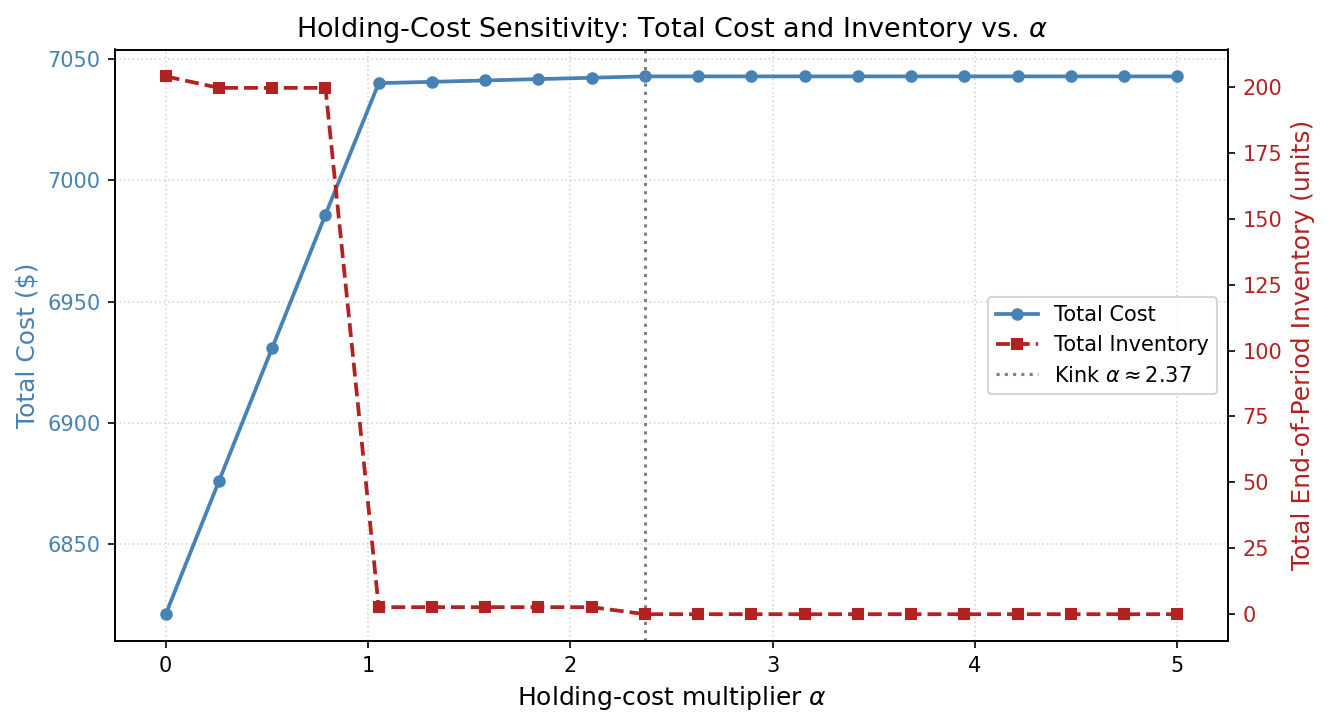
\includegraphics[width=0.86\textwidth]{fig_A2_holding_sensitivity.png}
  \caption{Total cost and end-of-period inventory vs.\ $\alpha$.}
  \label{fig:alpha}
\end{figure}

Up to $\alpha \approx 1.053$, the model holds around 200 units and cost climbs
steeply---unsurprisingly, since the same stock pile gets pricier to store.
At $\alpha \approx 1.053$ inventory falls to $\sim\!2.67$ units in a single
step, and at $\alpha \approx 2.37$ it reaches zero. Past that point the total
cost freezes at \$7\,042.92 no matter how large $\alpha$ gets.

\subsubsection*{Overtime cost ($\beta$ sweep)}

I swept $\beta \in [0.5, 4.0]$ over 15 points, replacing $c^{ov}_{m,t}$ with
$\beta \cdot c^{ov}_{m,t}$. Figure~\ref{fig:beta} shows the result.

\begin{figure}[H]
  \centering
  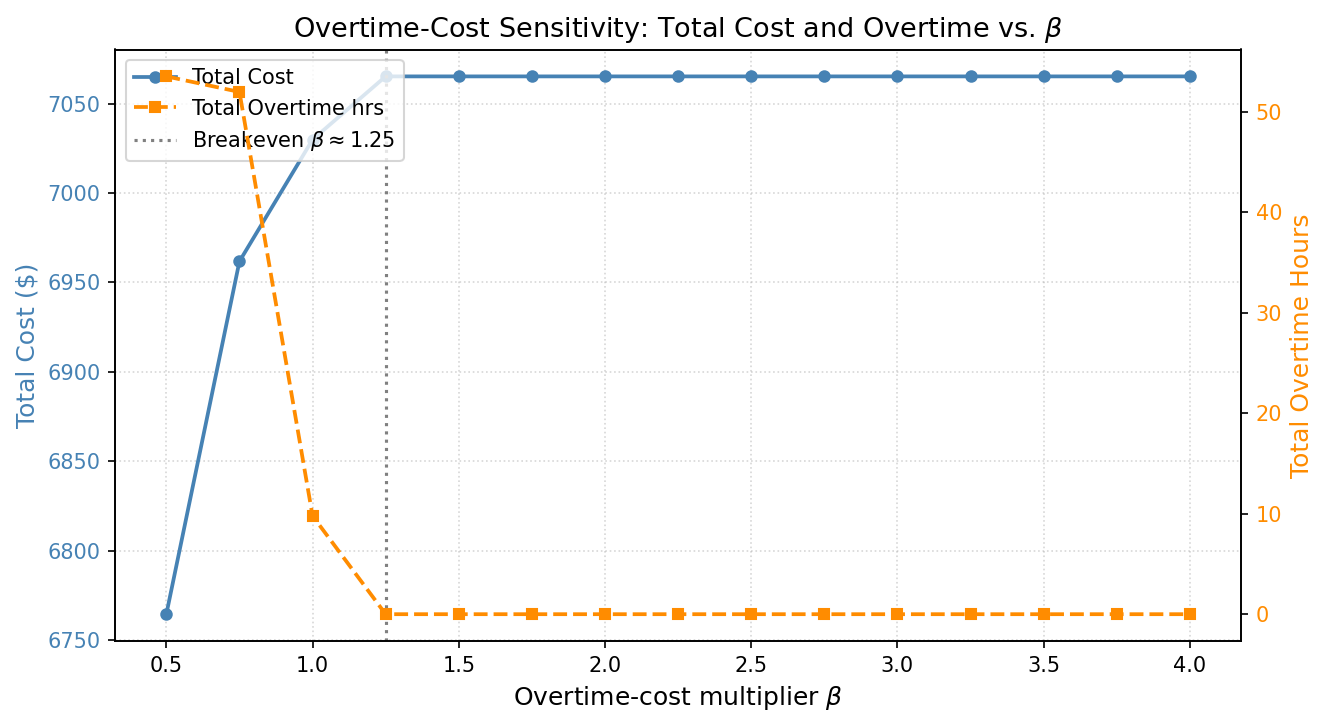
\includegraphics[width=0.86\textwidth]{fig_A3_overtime_sensitivity.png}
  \caption{Total cost and overtime hours vs.\ $\beta$.}
  \label{fig:beta}
\end{figure}

Overtime goes to zero at $\beta \approx 1.25$, which corresponds to
\$18.8/hr. After that the cost stabilises at \$7\,065.18. That's meaning that the overtime premium is high enought, so the model prefers to pay the activation fee and regular hours.

\subsection{Discussion}

\paragraph{Why does the holding-cost curve kink?}
not answered.

\paragraph{Is F2 used in all periods?}
No, only in periods~1 and~2. Keeping it off in periods~3 and~4 saves \$400
in activation fees. It's worth it because by period~3 the smoothing constraint
caps how much can be produced anyway (at most $1.25 \cdot X_{k,2}$), so the
extra F2 capacity would mostly go unused. F1 with under 10~hrs of overtime
is enough, and F2's higher unit cost ($c_0^{F2}=10$ vs.\ $c_0^{F1}=8$) makes
it a bad deal unless capacity is really tight.

\paragraph{What do the smoothing constraints actually do?}
Without them, the cheapest plan would be to dump everything into one period
on F1, pay one activation fee, and let the furnaces sit idle for the rest of
the horizon. The $\pm 25\%$ bounds prevent that: once production drops, it
can only recover slowly, which forces the model to keep furnaces running
through the whole planning period. From an operations standpoint that's
exactly right---you can't spin a steel furnace back up overnight.

% ==========================================================================
\section{Part B --- Minimum Lot Size and Setup Cost}
% ==========================================================================

\subsection{Mathematical formulation}

\paragraph{New binary variables.}
\[
  \delta_{m,k,t} \in \{0,1\}, \quad \forall\,m\in M,\ k\in K,\ t\in T.
\]
$\delta_{m,k,t}=1$ means furnace $m$ produces product $k$ in period
$t$, paying a setup; zero means it doesn't touch that product that period.

\paragraph{Coupling constraints.}
\begin{align}
  x_{m,k,t} & \leq M_{m,k,t}\;\delta_{m,k,t} \quad \forall m \in M, k \in K, t \in T \tag{B1} \label{eq:bigM} \\[2pt]
  x_{m,k,t} & \geq L_k\;\delta_{m,k,t} \quad \forall m \in M, k \in K, t \in T \tag{B2} \label{eq:minlot}
\end{align}

Constraint~\eqref{eq:bigM} forces $x_{m,k,t}=0$ whenever $\delta_{m,k,t}=0$
(Big-$M$ side).
Constraint~\eqref{eq:minlot} forces $x_{m,k,t} \geq L_k$ whenever
$\delta_{m,k,t}=1$ (minimum-lot side)

\paragraph{Modified objective.}
\[
  \min\;(\text{eq.}\ (1))\;+\;\sum_{m,k,t} SC_{m,k}\;\delta_{m,k,t},
  \qquad SC_{m,k}=50\;\forall\,(m,k).
\]

The eq.~(1) corresponds to the original objective.

\subsection{Results and comparison}

\begin{table}[H]
  \centering
  \caption{Part A vs.\ Part B --- summary}
  \begin{tabular}{lrr}
    \toprule
                       & Part A    & Part B    \\
    \midrule
    Optimal cost (\$)  & 7\,029.84 & 7\,637.39 \\
    Cost increase (\$) & ---       & $+607.56$ \\
    Setups paid        & ---       & 12 times  \\
    \bottomrule
  \end{tabular}
\end{table}

F1 sets up for A and C every period (8 setups), adds B in periods~3 and~4
(2 more), and F2 runs B only in periods~1--2 (2 setups): 12 total. Nothing
else was worth activating given the \$50 fee plus the minimum-lot commitment.

\begin{table}[H]
  \centering
  \caption{Aggregate production $X_{k,t}=\sum_m x_{m,k,t}$: Part A vs.\ Part B}
  \label{tab:comparison}
  \small
  \begin{tabular}{ccrrr}
    \toprule
    $k$ & $t$ & $X^{(A)}_{k,t}$ & $X^{(B)}_{k,t}$ & $\Delta$   \\
    \midrule
    A   & 1   & 82.53           & 74.09           & $-8.44$\;* \\
    A   & 2   & 61.90           & 67.14           & $+5.24$\;* \\
    A   & 3   & 46.43           & 50.35           & $+3.93$\;* \\
    A   & 4   & 45.14           & 44.42           & $-0.73$\;* \\
    \midrule
    B   & 1   & 63.27           & 63.27           & $0.00$     \\
    B   & 2   & 47.45           & 47.45           & $0.00$     \\
    B   & 3   & 35.59           & 35.59           & $0.00$     \\
    B   & 4   & 26.69           & 26.69           & $0.00$     \\
    \midrule
    C   & 1   & 36.11           & 32.39           & $-3.73$\;* \\
    C   & 2   & 38.87           & 40.48           & $+1.61$\;* \\
    C   & 3   & 29.15           & 30.36           & $+1.21$\;* \\
    C   & 4   & 21.86           & 22.77           & $+0.91$\;* \\
    \bottomrule
    \multicolumn{5}{l}{\small * changed from Part A.}
  \end{tabular}
\end{table}

Product~B doesn't change at all because neither furnace was below $L_B=20$ in
Part~A. Products~A and~C shift around because small sub-threshold lots get
dropped: the F2 lot for A in period~1 was $x_{F2,A,1}=11.42 < L_A=25$, so it
disappears and the missing volume gets redistributed to F1 over the remaining
periods---within the smoothing bounds.

\subsection{Discussion}

\paragraph{Why does Part B cost more?}
12 setups at \$50 accounts for \$600 of the \$607.56 gap. The remaining \$7.56
comes from the plan being slightly worse overall: some lots that were small but
efficient in Part~A now either have to be dropped or inflated to meet $L_k$,
and since the smoothing constraints link all four periods together, those
adjustments ripple forward and make the whole schedule a bit less efficient.
It's a small effect here, but with stricter lot sizes it would matter more.

\paragraph{Does a very large $SC_{m,k}$ necessarily reduce setups?}
Not in this case. The F2-B setups in periods~1 and~2 aren't there because they
were cheap---they're there because F1 is already running 50~hours on A and C
and has no capacity left for B.

\end{document}
